\iffalse
\let\negmedspace\undefined
\let\negthickspace\undefined
\documentclass[journal,12pt,twocolumn]{IEEEtran}
\usepackage{cite}
\usepackage{amsmath,amssymb,amsfonts,amsthm}
\usepackage{algorithmic}
\usepackage{graphicx}
\usepackage{textcomp}
\usepackage{xcolor}
\usepackage{txfonts}
\usepackage{listings}
\usepackage{enumitem}
\usepackage{mathtools}
\usepackage{float}
\usepackage{gensymb}
\usepackage{comment}
\usepackage[breaklinks=true]{hyperref}
\usepackage{tkz-euclide} 
\usepackage{listings}
\usepackage{gvv}                                        
\def\inputGnumericTable{}                                 
\usepackage[latin1]{inputenc}                                
\usepackage{color}                                            
\usepackage{array}          
\usetikzlibrary{positioning, arrows.meta}
\usepackage{longtable}                                       
\usepackage{calc}                                             
\usepackage{multirow}                                         
\usepackage{hhline}                                           
\usepackage{ifthen}                                           
\usepackage{lscape}
\usepackage{amsmath}
\newtheorem{theorem}{Theorem}[section]
\newtheorem{problem}{Problem}
\newtheorem{proposition}{Proposition}[section]
\newtheorem{lemma}{Lemma}[section]
\newtheorem{corollary}[theorem]{Corollary}
\newtheorem{example}{Example}[section]
\newtheorem{definition}[problem]{Definition}
\newcommand{\BEQA}{\begin{eqnarray}}
\newcommand{\EEQA}{\end{eqnarray}}
\newcommand{\define}{\stackrel{\triangle}{=}}
\theoremstyle{remark}
\newtheorem{rem}{Remark}
\begin{document}

\bibliographystyle{IEEEtran}
\title{GATE-BM-Q15}
\author{EE23BTECH11015 - DHANUSH V NAYAK$^{*}$% <-this % stops a space
}
\maketitle
\newpage
\bigskip
\renewcommand{\thefigure}{\arabic{figure}}
\renewcommand{\thetable}{\theenumi}
\textbf{Question:} Discrete signals $x\brak{n}$ and $y\brak{n}$ are shown below. The cross-correlation $r_{xy}\brak{0}$ is:
\begin{figure}[H]
    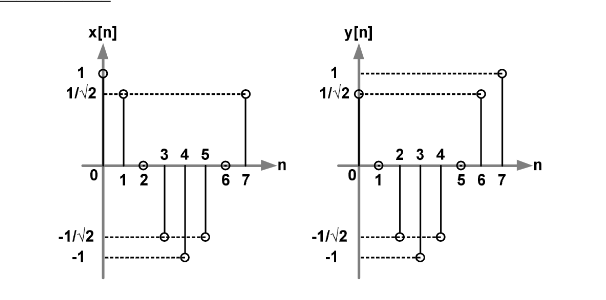
\includegraphics[width=1\columnwidth]{2022/BM/15/figs/question_BM_15.png}
    \caption{Question Figure}
    \label{fig:question_fig}
\end{figure}\hfill{(GATE BM 2022)}\\
\solution
\fi
\begin{table}[H]
\centering
\renewcommand\thetable{1}
\setlength{\extrarowheight}{9pt}
\resizebox{0.5\textwidth}{!}{
\begin{tabular}{|c|c|c|}
\hline
\textbf{Parameter} & \textbf{Description} & \textbf{Value} \\ \hline
$x\brak{n}$ & First Sequence & $x(n) = 
\begin{cases}
    0 & ; n < 0 \\
    \brak{1,\frac{1}{\sqrt{2}} , 0 ,-\frac{1}{\sqrt{2}},-1,-\frac{1}{\sqrt{2}},0,\frac{1}{\sqrt{2}}} & ; 0 \leq n \leq 7 \\
    0 & ; n > 7 \\
\end{cases}$   \\ \hline
$y\brak{n}$ &Second Sequence &$y(n) = 
\begin{cases}
    0 & ; n < 0 \\
    \brak{\frac{1}{\sqrt{2}} , 0 ,-\frac{1}{\sqrt{2}},-1,-\frac{1}{\sqrt{2}},0,\frac{1}{\sqrt{2}},1} & ; 0 \leq n \leq 7 \\
    0 & ; n > 7 \\
\end{cases}$  \\ \hline
$r_{xy}\brak{k}$& Cross-correlation & $\sum_{m=-\infty}^{\infty} x\brak{m}y\brak{m-k}$ \\ \hline 
\end{tabular}}
\caption{Parameter Table}
\label{tab:gate_bm_Q15}
\end{table}

It can be seen that :
\begin{align}
    y\brak{n} = x\brak{n+1}\label{eq:gate_bm_q15.1}
\end{align}
From \tabref{tab:gate_bm_Q15} :
\begin{align}
    r_{xy}\brak{k} &= \sum_{m=-\infty}^{\infty} x\brak{m}y\brak{m-k}\\
                &= x\brak{k} * y\brak{-k}
\end{align}
From \eqref{eq:gate_bm_q15.1}:
\begin{align}
    r_{xy}\brak{k} &= x\brak{k+1} * x\brak{-k}\\
                &= \sum_{n=-\infty}^{\infty} x\brak{n+1}x\brak{n+k} 
\end{align}
By definition of x\brak{n} from \tabref{tab:gate_bm_Q15}:
\begin{align}
     r_{xy}\brak{k} &= \sum_{n=0}^{6} x\brak{n+1}x\brak{n+k} \\
     r_{xy}\brak{0} &= \sum_{n=0}^{6} x\brak{n+1}x\brak{n} 
\end{align}
Using values from \figref{fig:question_fig}:
\begin{align}
    r_{xy}\brak{0} &= 2\sqrt{2}
\end{align}
\begin{figure}[H]
    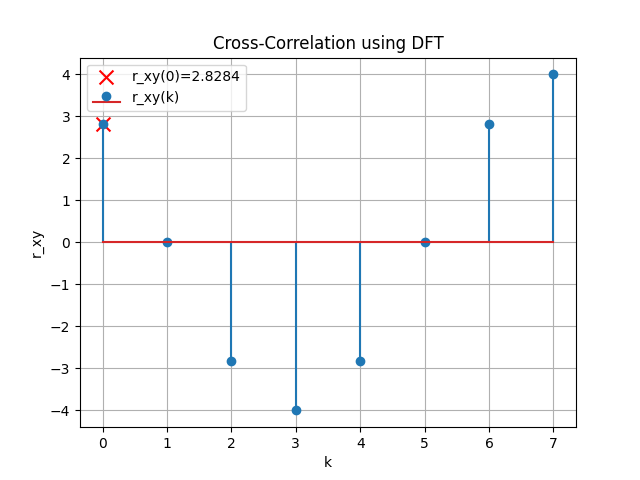
\includegraphics[width=1\columnwidth]{2022/BM/15/figs/cross-corelation.png}
    \caption{Verification of result by DFT}
    \label{fig:cross-corelation}
\end{figure}

%\end{document}

